\documentclass{article}

% if you need to pass options to natbib, use, e.g.:
%     \PassOptionsToPackage{numbers, compress}{natbib}
% before loading neurips_2018

% ready for submission
% \usepackage{neurips_2018}

% to compile a preprint version, e.g., for submission to arXiv, add add the
% [preprint] option:
%     \usepackage[preprint]{neurips_2018}

% to compile a camera-ready version, add the [final] option, e.g.:
     \usepackage[final]{nips_2018}

% to avoid loading the natbib package, add option nonatbib:
%     \usepackage[nonatbib]{neurips_2018}

% Packages to include
\usepackage{helvet}
\usepackage{tikz}
\usepackage{tikz-3dplot}
\usetikzlibrary{backgrounds,3d,shadings,shapes.misc,decorations.pathmorphing,shapes,calc}
%\usepackage{cite}
\usepackage{amssymb,amsmath}
\usepackage{booktabs} % for much better looking tables
\usepackage{mathtools}
%\usepackage{bbding}
\usepackage{graphicx} % support the \includegraphics command and options
\usepackage{subfig}
\usepackage{array} % for better arrays \left(eg matrices\right) in maths
\usepackage{paralist} % very flexible & customisable lists \left(eg. enumerate/itemize, etc.\right)
\usepackage{verbatim} % adds environment for commenting out blocks of text & for better verbatim
\usepackage[labelfont=bf,labelsep=space]{caption} % might need to comment this out in case of conflicts
\usepackage{sectsty} % might need to comment this out in case of conflicts
\usepackage{dblfloatfix} % might need to comment this out in case of conflicts
\usepackage[space]{grffile} % might need to comment this out in case of conflicts
\usepackage{url} % might need to comment this out in case of conflicts
\usepackage[toc]{appendix} % might need to comment this out in case of conflicts
\usepackage[titles,subfigure]{tocloft} % Alter the style of the Table of Contents. Might need to comment this out in case of conflicts
%\usepackage{geometry} % to change the page dimensions
%\geometry{letterpaper}
\usepackage[breakable, theorems, skins]{tcolorbox}
\usepackage{algorithm} % algorithms
\usepackage[noend]{algpseudocode} % algorithms
%\usepackage{hyperref}
\usepackage{pgfplots}
\usepackage{cancel}
\usepackage{bm}
\newcommand{\bs}[1]{\bm{\mathrm{#1}}}

% ---- Definitions ----

% Template for algorithms, source: https://tex.stackexchange.com/questions/163768/write-pseudo-code-in-latex

%\begin{algorithm}
%	\caption{Meta-pruning for weights} \label{alg1}
%	\begin{algorithmic}[1]
%		\Procedure{MyProcedure}{}
%		\State $\textit{stringlen} \gets \text{length of }\textit{string}$
%		\State $i \gets \textit{patlen}$
%		\BState \emph{top}:
%		\If {$i > \textit{stringlen}$} \Return false
%		\EndIf
%		\State $j \gets \textit{patlen}$
%		\BState \emph{loop}:
%		\If {$\textit{string}(i) = \textit{path}(j)$}
%		\State $j \gets j-1$.
%		\State $i \gets i-1$.
%		\State \textbf{goto} \emph{loop}.
%		\State \textbf{close};
%		\EndIf
%		\State $i \gets i+\max(\textit{delta}_1(\textit{string}(i)),\textit{delta}_2(j))$.
%		\State \textbf{goto} \emph{top}.
%		\EndProcedure
%	\end{algorithmic}
%\end{algorithm}



% Coloured boxes for highlighting text, e.g. for summaries, theorems, etc.
\DeclareRobustCommand{\colourbox}[2][gray!20]{%
	\begin{tcolorbox}[   %% Adjust the following parameters at will.
		breakable,
		left=0pt,
		right=0pt,
		top=0pt,
		bottom=0pt,
		colback=#1,
		colframe=#1,
		width=\dimexpr\textwidth\relax, 
		enlarge left by=0mm,
		boxsep=5pt,
		arc=0pt,outer arc=0pt,
		]
		#2
	\end{tcolorbox}
}


% ---- My definitions ----
%\DeclareMathOperator{\pv}{pv}
%\DeclareMathOperator{\sign}{sign}
%\DeclareMathOperator{\ber}{ber}
%\DeclareMathOperator{\bei}{bei}
%\newcommand{\vect}[1]{\mathbf{#1}}
%\newcommand{\nhat}{\mathbf{\hat{n}}}
\newcommand{\vect}[1]{\vec{#1}}
\newcommand{\nhat}{{\hat{n}}}
\newcommand{\nvec}{{\hat{n}}}
\newcommand{\ver}[1]{\hat{#1}}
%\newcommand{\matr}[1]{\mathbf{#1}}
\newcommand{\matr}[1]{\bs{#1}}
\newcommand{\abs}[1]{\left \lvert #1 \right\rvert }
\newcommand{\norm}[1]{ \left \lVert #1 \right \rVert} 
%\newcommand{\pvint}{\pv\!\!\int}
\newcommand{\pvint}{\dashint}
\newcommand{\intR}{\int_{-\infty}^{+\infty}}
\newcommand{\pvintR}{\pvint_{-\infty}^{+\infty}}
\newcommand{\laplace}[1]{\mathscr{L}\{#1\}}
\newcommand{\ilaplace}[1]{\mathscr{L}^{-1}\{#1\}}
\newcommand{\blaplace}[1]{\mathscr{L}_b\{#1\}}
\newcommand{\fourier}[1]{\mathscr{F}\{#1\}}
\newcommand{\ifourier}[1]{\mathscr{F}^{-1}\{#1\}}
\renewcommand{\Re}[1]{\mathbb{R}\mathrm{e}\left \{#1\right\} }
\renewcommand{\Im}[1]{\mathbb{I}\mathrm{m}\left \{#1\right\} }
\newcommand{\Real}{\mathbb{R}}
\newcommand{\Complex}{\mathbb{C}}
% Sets
\newcommand{\complem}[1]{#1^{\rm C}}
\newcommand{\expon}[1]{\operatorname{e}^{\,#1}}
\newcommand{\ns}{\!\!\!\!}
\newcommand{\pref}[1]{(\ref{#1})}
\newcommand{\junk}[1] {}
\newcommand{\missing}[1]{\vspace*{\parskip}
			\centerline{\framebox{\begin{minipage}{0.9\columnwidth}{\large\bf\noindent #1}
				\end{minipage}}}
			\vspace*{\parskip}}


% Principal value integral sign
\def\Xint#1{\mathchoice
{\XXint\displaystyle\textstyle{#1}}%
{\XXint\textstyle\scriptstyle{#1}}%
{\XXint\scriptstyle\scriptscriptstyle{#1}}%
{\XXint\scriptscriptstyle\scriptscriptstyle{#1}}%
\!\int}
\def\XXint#1#2#3{{\setbox0=\hbox{$#1{#2#3}{\int}$}
\vcenter{\hbox{$#2#3$}}\kern-.5\wd0}}
\def\ddashint{\Xint=}
\def\dashint{\Xint-}

\newcommand*\widebar[1]{%
  \hbox{%
    \vbox{%
      \hrule height 0.5pt % The actual bar
      \kern0.3ex%         % Distance between bar and symbol
      \hbox{%
        \kern-0.05em%      % Shortening on the left side
        \ensuremath{#1}%
        \kern-0.05em%      % Shortening on the right side
      }%
    }%
  }%
} 


\renewcommand{\epsilon}{\varepsilon}

\newcommand{\dbd}[2]{\ensuremath{\dfrac{d#1}{d#2}}}
\newcommand{\ddt}[1]{\ensuremath{\dfrac{d#1}{dt}}}
\newcommand{\ddx}[1]{\ensuremath{\dfrac{d#1}{dx}}}
\newcommand{\ddy}[1]{\ensuremath{\dfrac{d#1}{dy}}}
\newcommand{\ddz}[1]{\ensuremath{\dfrac{d#1}{dz}}}

\newcommand{\pardt}[1]{\ensuremath{\dfrac{\partial#1}{\partial t}}}
\newcommand{\pardx}[1]{\ensuremath{\dfrac{\partial#1}{\partial x}}}
\newcommand{\pardy}[1]{\ensuremath{\dfrac{\partial#1}{\partial y}}}
\newcommand{\pardz}[1]{\ensuremath{\dfrac{\partial#1}{\partial z}}}

\newcommand{\pardtsq}[1]{\ensuremath{\dfrac{\partial^2#1}{\partial t^2}}}
\newcommand{\pardxsq}[1]{\ensuremath{\dfrac{\partial^2#1}{\partial x^2}}}
\newcommand{\pardysq}[1]{\ensuremath{\dfrac{\partial^2#1}{\partial y^2}}}
\newcommand{\pardzsq}[1]{\ensuremath{\dfrac{\partial^2#1}{\partial z^2}}}

\newcommand{\curl}[1]{\ensuremath{\nabla\times\bs{#1}}}
\newcommand{\tensor}[1]{\ensuremath{\bar{\bar{#1}}}}

\newcommand{\figref}[1]{Figure~\ref{#1}}
\newcommand{\algoref}[1]{Algorithm~\ref{#1}}
\newcommand{\secref}[1]{Section~\ref{#1}}
\newcommand{\tabref}[1]{Table~\ref{#1}}

\newcommand{\opL}{\mathcal{L}} % L operator
\newcommand{\opK}{\mathcal{K}} % K operator

% Theorems, laws, definitions environments
\newtheorem{defn}{Definition}
\newtheorem{thm}{Theorem}
\newtheorem{exm}{Example}
\newtheorem{rmk}{Remark}


\usepackage{listings}
\usepackage{color}

\definecolor{mygreen}{RGB}{28,172,0} % color values Red, Green, Blue
\definecolor{mylilas}{RGB}{170,55,241}

\lstset{language=Matlab,%
	%basicstyle=\color{red},
	basicstyle=\ttfamily,
	breaklines=true,%
	morekeywords={matlab2tikz},
	%keywordstyle=\color{blue},%
	morekeywords=[2]{1}, keywordstyle=[2]{\color{black}},
	identifierstyle=\color{black},%
	stringstyle=\color{mylilas},
	commentstyle=\color{mygreen},%
	showstringspaces=false,%without this there will be a symbol in the places where there is a space
	numbers=left,%
	numberstyle={\tiny \color{black}},% size of the numbers
	numbersep=9pt, % this defines how far the numbers are from the text
	emph=[1]{for,end,break},emphstyle=[1]\color{blue}, %some words to emphasise
	%emph=[2]{word1,word2}, emphstyle=[2]{style},    
}



% For algorithms
\makeatletter
\def\BState{\State\hskip-\ALG@thistlm}
\makeatother

\usepackage[utf8]{inputenc} % allow utf-8 input
\usepackage[T1]{fontenc}    % use 8-bit T1 fonts
%\usepackage{hyperref}       % hyperlinks
\usepackage{url}            % simple URL typesetting
\usepackage{booktabs}       % professional-quality tables
\usepackage{amsfonts}       % blackboard math symbols
\usepackage{nicefrac}       % compact symbols for 1/2, etc.
\usepackage{microtype}      % microtypography

\title{Network Pruning Based on Multiple Datasets for Performance and Generalization}

% The \author macro works with any number of authors. There are two commands
% used to separate the names and addresses of multiple authors: \And and \AND.
%
% Using \And between authors leaves it to LaTeX to determine where to break the
% lines. Using \AND forces a line break at that point. So, if LaTeX puts 3 of 4
% authors names on the first line, and the last on the second line, try using
% \AND instead of \And before the third author name.

\author{%
  Adriana~Salcedo\\
  Department of Medical Biophysics\\
  University of Toronto\\
  Toronto, ON M5S 1A1\\
  \texttt{a.salcedo@mail.utoronto.ca} \\
  % examples of more authors
   \And
   Shashwat~Sharma\\
   Edward S.~Rogers~Sr. Department of Electrical \& Computer Engineering \\
   University of Toronto\\
   Toronto, ON M5S 1A1\\
   \texttt{shash.sharma@mail.utoronto.ca} \\
  % \AND
  % Coauthor \\
  % Affiliation \\
  % Address \\
  % \texttt{email} \\
  % \And
  % Coauthor \\
  % Affiliation \\
  % Address \\
  % \texttt{email} \\
  % \And
  % Coauthor \\
  % Affiliation \\
  % Address \\
  % \texttt{email} \\
}

\begin{document}
% \nipsfinalcopy is no longer used

\maketitle

\begin{abstract}
  The abstract paragraph should be indented \nicefrac{1}{2}~inch (3~picas) on
  both the left- and right-hand margins. Use 10~point type, with a vertical
  spacing (leading) of 11~points.  The word \textbf{Abstract} must be centered,
  bold, and in point size 12. Two line spaces precede the abstract. The abstract
  must be limited to one paragraph.
\end{abstract}

\section{Introduction}

Modern neural networks tend to be immensely large with several millions of connections and weights. The memory and energy requirements for deploying such networks is significant, and constantly growing with the complexity of state-of-the-art networks. Although having a large number of trainable parameters is beneficial to network accuracy, it was shown by \citet{NIPS_learning_weights_pruning}, \citet{OBD} and \citet{OBS} that the impact of some parameters is negligible in comparison with others. Successful identification and removal (``pruning'') of such parameters would lead to smaller and faster networks, which in turn would significantly reduce the computational cost at test time. The goal of most pruning algorithms is to achieve computational advantages without an appreciable impact on accuracy. The importance and relevance of network pruning was recently highlighted via MorphNet, proposed by \citet{morphnet} at Google to optimize existing networks through pruning.

It was argued by \citet{prune_transfer_learning} that pruning can also be applied in the context of transfer learning, for generalization of a trained network to related datasets. Improved ability of networks to generalize as a result of pruning was also achieved by \citet{prune_for_architecture}. However, these approaches target networks that have been trained on a single dataset. In contrast, the concept of learning the hyperparameters of a network by using multiple datasets, known as ``meta-learning", has also been proposed by \citet{metalearning1}. To the best of our knowledge, the meta-learning concept has not been applied in the context of network pruning.

The above points motivate the main idea proposed in this work: designing pruning methodologies that specifically target improved generalization of a given network, by leveraging multiple datasets during training. The goal is to optimize existing networks not only to be faster and smaller, but also to improve their ability to generalize. We first implement and study some simple and commonly-used pruning strategies and analyze their impact on network size, speed and accuracy. We then discuss and implement a simple meta-learning algorithm and study its performance. Finally, we combine the pruning strategies with the meta-learning algorithm to introduce a proof-of-concept ``meta-pruning'' methodology.

\section{Formal Description}

\subsection{A Survey on Simple Pruning Algorithms}

\subsubsection{Masking of Classifier Layers Based on a Threshold} \label{maskClass}

\subsubsection{Learned Masking of Classifier Layers} \label{maskClassL0}

\subsubsection{Pruning Convolution Filters} \label{PruneFilter}

One method to prune convolutional layers is to reduce the number of output channels in each layer, which involves reducing the size of associated weight matrices. This impacts not only the convolution layer being pruned, but also the number of input channels in the next layer of the network. This approach was proposed by \cite{prune_transfer_learning}, and has since been implemented via open-source code provided by \cite{jacobgilblog}. However, this implementation only allows for pruning a single output channel at a time. We have implemented a version of this technique that allows pruning out several filters simultaneously, greatly improving the efficiency of aforementioned the code.

Although a relatively sophisticated strategy for picking pruned channels was presented by \cite{prune_transfer_learning}, in our implementation we use two simple metrics to decide which channels are to be pruned: the 2-norm of the layer's activations, and the 2-norm of weights. In each case, pruning occurs after every $N_i$ epochs, until training is complete. The number of output channels to prune, $N_p$, is set via the hyperparameter $p$, which is a percentage of the total available parameters in that network, $N_\mathrm{total}$:
\begin{align}
	N_p = \mathrm{round} \left(\dfrac{p}{100}N_\mathrm{total}\right). \label{eqNp}
\end{align}
In the activation-based approach, the activations of each layer are accumulated over the $N_i$ epochs preceding a single pruning pass via the function \texttt{TrackConv2DNorms}. This is done as follows: at each training iteration, we compute the 2-norm of the activations of each layer, across all of the input data dimensions (function \texttt{ComputeConv2DActNorms}). The output of this is a vector whose size is the number of output channels of a particular layer, and one such vector is constructed for each convolution layer. These vectors represent the strength of the activations of each filter. Optionally, these vectors can be normalized to their maximum values to ensure that every set of $N_i$ epochs is equally represented.

The new activation norm vectors computed at each iteration are added to the previously stored vectors. Every $N_i$ epochs, we look at the accumulated activation vector and extract the indices corresponding to the $N_p$ smallest activations (function \texttt{PruneAllConv2DLayers}). This tells us the $N_p$ filters of each layer which had, on average, the weakest activations over the last $N_i$ epochs. Those filters are then pruned away, and the old model is replaced with the updated, smaller model (function \texttt{PruneConvLayers}). At this stage, the accumulated activation norm vectors are reset to their initial state, ready to start accumulating activations for the next $N_i$ epochs.

When pruning based on weights, the strategy is the same as above, except that rather than accumulating activations, we accumulate the 2-norms of the weight matrices themselves. The 2-norms are computed over the input channel dimension, and over the kernel of each filter (function \texttt{ComputeConv2DWeightNorms}). Again, this yields, for each layer, a vector containing 2-norms corresponding to the weights of each output channel. This can also be optionally normalized to the maximum value in each vector. Every $N_i$ epochs, these accumulated vectors are used to prune away the weakest $N_p$ filters.

The methodology described above is summarized in \algoref{FilterPruneBasic}.
The results of both methods in comparison to the baseline (no pruning) are discussed below.

\begin{algorithm}[t]
	\caption{Helper functions for iterative convolution filter pruning - single dataset} \label{FilterPruneBasic}
	\begin{algorithmic}[1]
		\Function{ComputeConv2DWeightNorms}{${\mathrm{model}, \matr{n}_w}$}
			\For {all $i$ in $\textit{convolution layers of }\mathrm{model}$}
				\State $\widetilde{\matr{n}}_{w,i} \gets \textit{2-norm of weights of layer }i\textit{ across dims 1, 2, 3}$
				\State $\widetilde{\matr{n}}_{w,i} \gets \widetilde{\matr{n}}_{w,i} / \max\abs{\widetilde{\matr{n}}_{w,i}} \textit{ (optional)}$
				\State $\matr{n}_{w,i} \gets \textit{append }\widetilde{\matr{n}}_{w,i}$
			\EndFor
			\State \Return $\matr{n}_{w,i}$
		\EndFunction
		\\
	%	
		\Function{ComputeConv2DActNorms}{${\mathrm{model}, \matr{n}_a}$}
			\For {all $i$ in $\textit{convolution layers of }\mathrm{model}$}
				\State $\widetilde{\matr{n}}_{a,i} \gets \textit{2-norm of activations of layer }i\textit{ across dims 0, 2, 3}$
				\State $\widetilde{\matr{n}}_{a,i} \gets \widetilde{\matr{n}}_{a,i} / \max\abs{\widetilde{\matr{n}}_{a,i}} \textit{ (optional)}$
				\State $\matr{n}_{a,i} \gets \textit{append }\widetilde{\matr{n}}_{a,i}$
			\EndFor
			\State \Return $\matr{n}_{a,i}$
		\EndFunction
%
	\end{algorithmic}
\end{algorithm}


\begin{algorithm}[t]
	\caption{Computational functions for iterative convolution filter pruning - single dataset} \label{FilterPruneComps}
	\begin{algorithmic}[1]
		\Function{PruneConvLayers}{${\matr{l}_\mathrm{idx}, \matr{f}_\mathrm{idx}, \mathrm{model}}$}
			\State $\matr{c}_\mathrm{idx} \gets \matr{l}_\mathrm{idx}^\mathrm{th}\textit{ conv layer of } \mathrm{model}$
			\State $\matr{w}_0 \gets \textit{weights of  } \matr{c}_\mathrm{idx}$
			\State $\matr{w}_0 \gets \textit{delete entries corresponding to filters in }\matr{f}_\mathrm{idx}$
			\State $\matr{c}_\mathrm{idx} \gets \textit{copy updated weights }\matr{w}_0$
			\State $\mathrm{model} \gets \textit{updated conv layer }\matr{c}_\mathrm{idx} \textit{ at layer }\matr{l}_\mathrm{idx}$
			\State \Return $\mathrm{model}$
		\EndFunction
		\\
		%		
		\Function{PruneAllConv2DLayers}{${\matr{n}_{a}, \matr{n}_{w}, N_p, \mathrm{model}}$}
		\For {all $i$ in $\textit{convolution layers of }\mathrm{model}$}
			\If {\textit{activation-based pruning}}
				\State $\matr{n}_{i} \gets \matr{n}_{a,i}$
			\ElsIf {\textit{weight-based pruning}}
				\State $\matr{n}_{i} \gets \matr{n}_{w,i}$
			\EndIf
			\State $\matr{f}_\mathrm{idx,i} \gets \textit{indices of bottom $N_p$ elements of }\matr{n}_{i}$
			\State $\mathrm{model} \gets$ \Call{PruneConvLayers}{${i, \matr{f}_\mathrm{idx,i}, \mathrm{model}}$}
		\EndFor
%		
		\State \Return $\mathrm{model}$
		\EndFunction
		%
	\end{algorithmic}
\end{algorithm}

\begin{algorithm}[t]
	\caption{Driver functions for iterative convolution filter pruning - single dataset} \label{FilterPruneDrivers}
	\begin{algorithmic}[1]
			\Function{TrainModel}{$\mathrm{model}, \mathrm{input}, N_i, N_p$}
			\For {all $i$ in $\mathrm{input}$}
				\State $\matr{n}_{a} +\gets$ \Call{ComputeConv2DActNorms}{${\mathrm{model}, \matr{n}_{a}}$}
				\State $\matr{n}_{w} +\gets$ \Call{ComputeConv2DWeightNorms}{${\mathrm{model}, \matr{n}_{w}}$}
				\If {$i \% N_i == 0$}
					\State $\mathrm{model} \gets$ \Call{PruneAllConv2DLayers}{${\matr{n}_{a}, \matr{n}_{w}, N_p, \mathrm{model}}$}
					\State $\matr{n}_{a} \gets \textit{reset}$
					\State $\matr{n}_{w} \gets \textit{reset}$
				\EndIf
			\EndFor
			%		
			\State \Return $\mathrm{model}$
		\EndFunction\\
%		
		\State $\mathrm{model} \gets \textit{VGG16}$
		\State $p \gets 5$
		\State $N_p \gets \textit{value as per \eqref{eqNp}}$
		\State $N_i \gets 7$
		\State $\mathrm{input} \gets \textit{sample 10\% of data from CIFAR-10}$
		\While {$i < 50$}
			\State $\mathrm{model} \gets $ \Call{TrainModel}{$\mathrm{model}, \mathrm{input}, N_i, N_p$}
		\EndWhile
		%
	\end{algorithmic}
\end{algorithm}


\begin{algorithm}[t]
	\caption{Driver function for meta convolution filter pruning - multiple datasets} \label{FilterPruneDriverMeta}
	\begin{algorithmic}[1]	
		\State $\mathrm{model} \gets \textit{VGG16}$
		\State $p \gets 5$
		\State $N_p \gets \textit{value as per \eqref{eqNp}}$
		\State $N_i \gets 7$
		\State $\mathrm{datasets} \gets \textit{dataloaders for several different datasets, in this case $8$}$
		\State $j \gets 0$
		\While {$i < 50$}
			\If {$i \% N_i == 0$}
				\State $\mathrm{input} \gets \textit{sample 10\% of data from $\mathrm{dataset}$ }j$
				\State $j \gets j + 1$
			\EndIf
			\State $\mathrm{model} \gets $ \Call{TrainModel}{$\mathrm{model}, \mathrm{input}, N_i, N_p$}
		\EndWhile
		%
	\end{algorithmic}
\end{algorithm}

\subsection{Pruning with Multiple Datasets}

\subsubsection{Intersection Pruning of Classifier Layers Based on a Threshold} \label{intersectPruneClass}


\subsubsection{Meta-Pruning Classifier Layers} \label{metaPruneClass}


\subsubsection{Intersection Pruning of Convolution Filters} \label{intersectPruneFilter}

Our initial attempt at applying meta-pruning to convolution filters by using the L0 norm-based masking yielded significantly deteriorated training results. At the same time, the results obtained by weight- or activation-based pruning (rather than learned masking) were comparable to the baseline case of no pruning, discussed further in \secref{PruneFilterRes}. These observations motivated us to leverage multiple datasets in the sense of intersection pruning, as described earlier in \secref{intersectPruneClass}, to prune convolution layers. This method proceeds exactly as the description in \secref{PruneFilter}, except that after every $N_i$ epochs, the input data is resampled from a different dataset. The associated algorithm is summarized in \algoref{FilterPruneDriverMeta}.


\section{Related Work}


\section{Demonstration}

The existing PyTorch implementation of VGG16 was used as the model to prune in all tests conducted in this work. The optimizer and other settings used were the same in all tests conducted, and can be found in accompanying code.

\subsection{A Study on Simple Pruning Algorithms}

In this study, the model was trained only on CIFAR-10 images. Due to limitations in computational resources available via Google Colab, only 2-10\% of the total available training images were used, to get results in a reasonable amount of time. Since the main point to be studied here is the performance of a pruned network compared to an unpruned network, we are only interested in the relative loss and accuracy. Thus, using the partial dataset is justified.

\subsubsection{Masking of Classifier Layers Based on a Threshold}

\subsubsection{Learned Masking of Classifier Layers}

\subsubsection{Pruning Convolution Filters} \label{PruneFilterRes}

Both activation-based and weight-based filter pruning approaches were studied. Since pruning is generally applied to fine-tune pre-trained network, the pre-trained version of VGG16 was used in this study. Pre-training was done on ImageNet, and the fine-tuning while pruning was done on CIFAR-10 images. In each case, pruning was performed after every $N_i = 7$ epochs. The percentage of filters pruned each time was $5$\%. Since the same settings were used in both methods, the number of filters pruned was the same in both cases. At the start, the model contained a total of $4224$ filters. After $49$ epochs, $3136$ filters survived, thus reducing the network size to $74$\% of its original size, not counting the classifier layers. Although the training time is usually not something that is critical to reduce, it is worth noting that training becomes faster as it proceeds due to the decreasing size of the network. The first $7$ epochs took $19$ minutes on average to train, while the last $7$ epochs took $14$ minutes on average. This is an indication of the expected improvement in network agility.

Training and validation results for both pruning approaches are shown in \figref{pruneFiltersSingle}. The top row shows accuracy, while the bottom row shows loss. The first column on the left shows baseline results with no pruning. The second column shows activation-based filter pruning results, and the third column shows weight-based pruning results. It was found that normalization of the accumulated weight or activation vectors does not have a significant impact on the results, so we only show results for the case when the vectors are not normalized.

The figures show that the both filter pruning approaches studied here decrease training accuracy compared to the baseline model by approximately $10$\% on average. However, the validation accuracy is only $3$--$5$\% lower than that obtained with the baseline model, on average. Furthermore, it is clear that the difference between training and validation accuracy in the baseline model is approximately $10$\%, while in the pruned networks, both training and validation performance are quite well balanced with respect to one another. This is an indicator that, as hypothesized, the pruned network has the potential to generalize better than the original network. The pruned network loss and accuracy are much less stable over epochs than the original model, which could perhaps be improved with more gradual pruning, or more sophisticated algorithms for choosing which filters to prune.
%The second column shows results when the weight and activation vectors are \emph{not} normalized, while the second one shows results for when they \emph{are} normalized.
\begin{figure}[!t]
	\centering
	\subfloat[][]
	{\hspace{-11mm}
		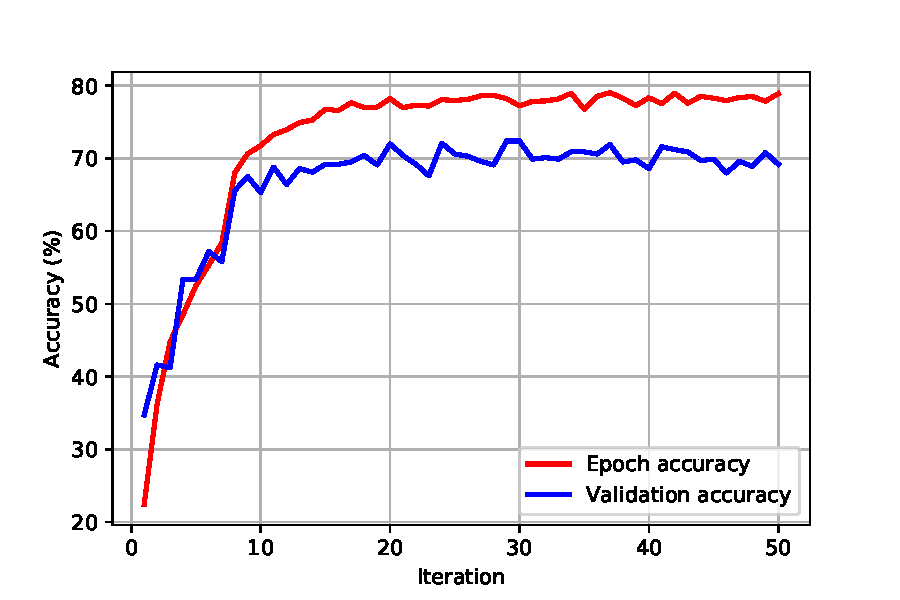
\includegraphics[width=6cm]{./results/baseline_pre_out_1_in_50_cifar10_10percent_acc.pdf}
	}
	\subfloat[][]
	{\hspace{-7mm}
		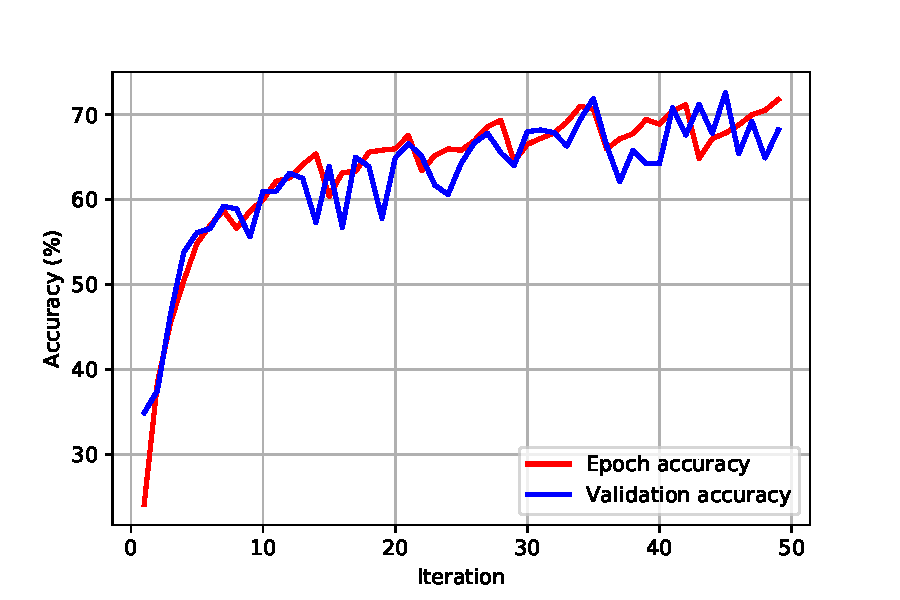
\includegraphics[width=6cm]{./results/pPruneActNoNorm5_pre_out_7_in_7_cifar10_10percent_acc.pdf}
	}
	\subfloat[][]
	{\hspace{-7mm}
		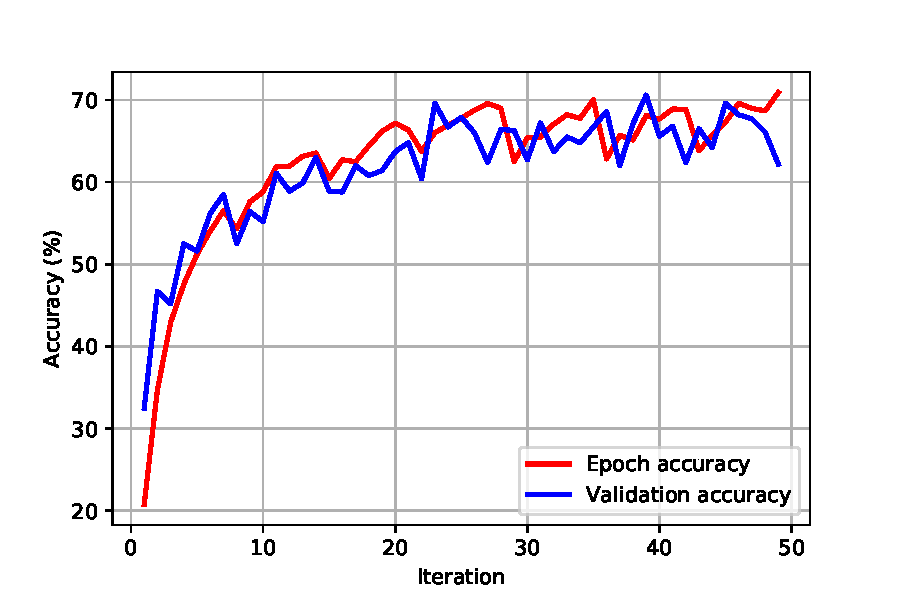
\includegraphics[width=6cm]{./results/pPruneWeightNoNorm5_pre_out_7_in_7_cifar10_10percent_acc.pdf}
	}\\[-5mm]
	\subfloat[][]
	{\hspace{-11mm}
		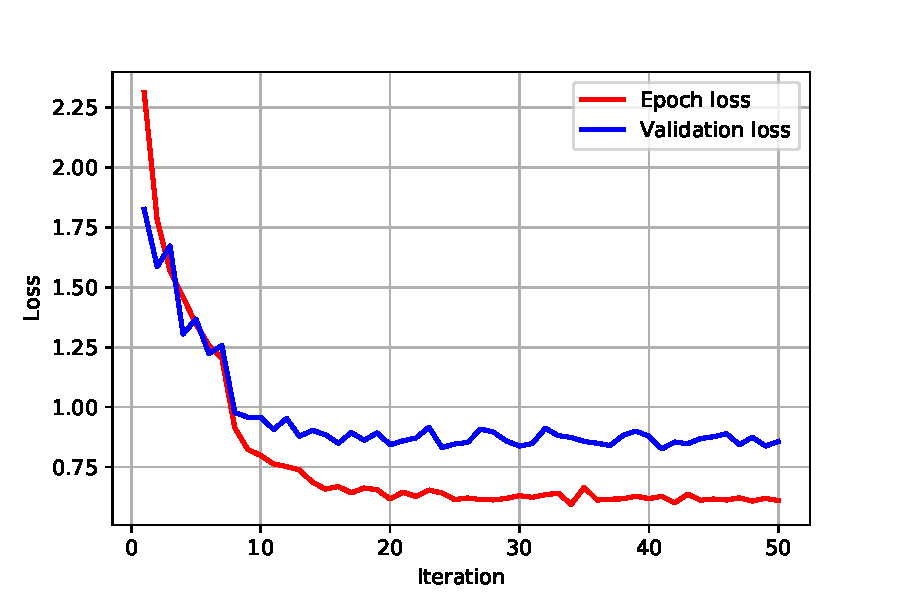
\includegraphics[width=6cm]{./results/baseline_pre_out_1_in_50_cifar10_10percent_loss.pdf}
	}
	\subfloat[][]
	{\hspace{-7mm}
		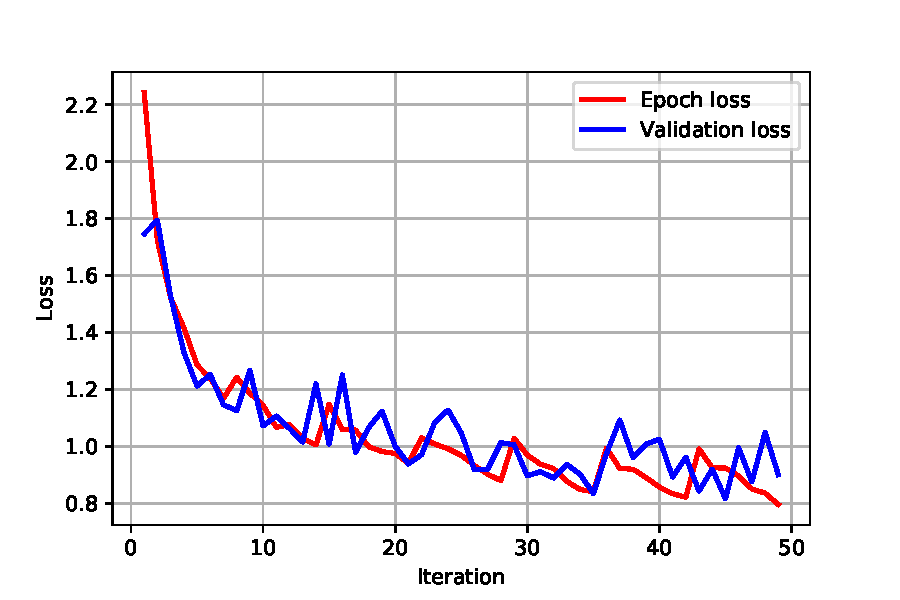
\includegraphics[width=6cm]{./results/pPruneActNoNorm5_pre_out_7_in_7_cifar10_10percent_loss.pdf}
	}
	\subfloat[][]
	{\hspace{-7mm}
		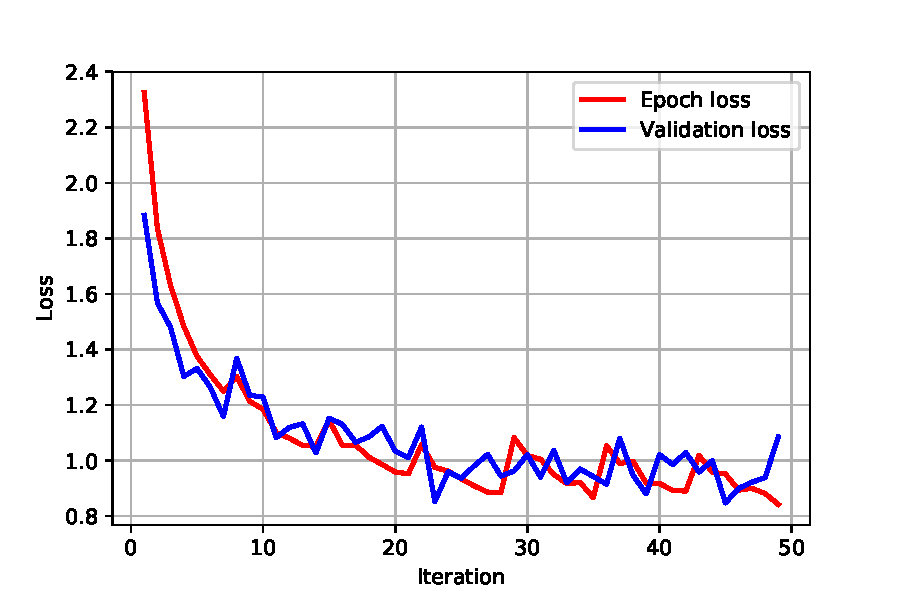
\includegraphics[width=6cm]{./results/pPruneWeightNoNorm5_pre_out_7_in_7_cifar10_10percent_loss.pdf}
	}
	\caption{Accuracy and loss of pre-trained VGG16 during fine-tuning. All layers were fine-tuned on 10\% of CIFAR-10 data ($4000$ training images, $1000$ validation images) for $50$ epochs. Top row: accuracy. Bottom row: loss. Left column: baseline model with no pruning. Middle column: activation-based pruning of $5$\% of all filters every $7$ epochs. Right column: weight-based pruning of $5$\% of all filters every $7$ epochs.}
	\label{pruneFiltersSingle}
\end{figure}


%\begin{itemize}
%	
%	\item Activation-Based Pruning
%	Baseline time: 136m 58s
%	Times: 19m 34s   19m 2s   17m 58s   16m 39s   16m 3s   15m 14s   13m 55s, total: 
%	Filters: 4224.0   4020.0   3822.0   3637.0   3458.0   3294.0   3136.0
%	
%	\item Weight-Based Pruning
%	Times: 19m 42s   19m 10s   18m 8s   16m 46s   16m 10s   15m 20s  14m 2s
%	Filters: 
%	
%\end{itemize}

\subsection{Pruning with Multiple Datasets}

\subsubsection{Intersection Pruning of Classifier Layers Based on a Threshold}


\subsubsection{Meta-Pruning Classifier Layers}


\subsubsection{Intersection Pruning of Convolution Filters}


\section{Limitations}


\section{Conclusions}


\section{List of Contributions}


\ \\ 
\ \\
\ \\
**************** Dumping figures here for now ****************





\ \\ 
\ \\
\ \\

**************** Text below is copied from proposal ****************

A variety of pruning algorithms have been proposed, many of which apply to convolutional neural networks. Some remove individual weights (leading to sparse weight matrices) while others remove entire filters, channels or layers. Units may be removed based on many criteria, including their magnitude, their contribution to the final loss (approximated through their gradients), and information criteria such as entropy~\citet{NIPS_learning_weights_pruning, prune_transfer_learning, prune_entropy, prune_slimming}.  Pruning may be applied towards a human-defined architecture (e.g. removing a certain proportion of weights in each layer)~\citet{prune_nisp} or help determine the final architecture autonomously~\citet{prune_thinet}. 

\section{Goals}





After each dataset sample, only connections that survive pruning and thus contribute to the final loss will be retained.  At the beginning of each dataset sample, weights will be initialized with the value of the updated weights in the previous sample. We hypothesize that this approach will result in weights that are important for a broad set of related tasks. 

It has been suggested~\citet{prune_for_architecture} that pruning can also improve algorithm efficiency by virtue of the resulting architecture, rather than just the resulting weights. Therefore, we will also assess a modified meta-pruning algorithm that only retains the architecture, and not the weights, across datasets:



We hypothesize that this approach will result in architectures that are more generalizable and efficient than the full model. Comparing the two approaches in algorithms 1 and 2 will illuminate the relative contributions of the weights and the architecture to the value of pruning for generalizability. 

\section{Methods}

We will first select a relatively simple pruning algorithm that can be adapted to the meta-pruning approach described above, as a proof of concept. Since pruning studies to date have largely focused on convolutional neural networks, we will develop our algorithm in the context of image recognition, initially working with the CIFAR-100 data. For the initial model, we will use VGGNet due to its simple architecture and expand to ResNet if time allows. To assess our algorithms' baseline performance, we will use test images which have the same categories as the training images. We will then assess our algorithms' capacity to generalize using a test set that contains a distinct set of categories from the training set. We will use cross entropy loss and assess the algorithms' performance by comparing its classification accuracy to the accuracy of the full model, as well as a reduced model with the same number of connections but where connections are randomly dropped. We will also compare the training time, memory requirements, and the number of retained parameters to assess the algorithms' efficiency and quantify the amount of compression achieved.

An important consideration in the proposed algorithms is the consequence of pruning to backpropagation. Particularly in algorithm 1, depending on the order in which operations are applied, special care must be taken to ensure that gradients are computed correctly for the pruned model, at each outer iteration. One way to circumvent the issue is to recompute gradients every time the model is updated via pruning. However, it may be possible to do this more intelligently by applying advanced techniques for gradients of discrete problems. This will be an area to explore, if time permits.

\begin{algorithm}[t]
	\caption{Meta-pruning for weights} \label{alg1}
	\begin{algorithmic}[1]
		\State $\theta \gets \textit{Random initialization}$
		\For {all $D$ in collection of datasets $\mathcal{D}$}
		\State $T \gets \textit{Sample tasks from dataset } D$
		\For {all $i$ in $T$}
		\State $G_i \gets \nabla_{\theta,i} \mathcal{L} \left(f_{\theta,i}\right)$
		\State $\theta_i \gets \theta_i - \beta G_i$
		\EndFor
		\State $\theta \gets \textit{Pruned and fine-tuned } \theta$
		\EndFor
	\end{algorithmic}
\end{algorithm}

\begin{algorithm}[t]
	\caption{Meta-pruning for architecture} \label{alg2}
	\begin{algorithmic}[1]
		%		\State $\theta \gets \textit{Random initialization}$
		\For {all $D$ in collection of datasets $\mathcal{D}$}
		\State $\theta \gets \textit{Random initialization}$
		\State $T \gets \textit{Sample tasks from dataset } D$
		\For {all $i$ in $T$}
		\State $G_i \gets \nabla_{\theta,i} \mathcal{L} \left(f_{\theta,i}\right)$
		\State $\theta_i \gets \theta_i - \beta G_i$
		\EndFor
		\State $\theta \gets \textit{Pruned } \theta$
		\EndFor
	\end{algorithmic}
\end{algorithm}

\section{Nice-to-haves}

There are several additional analyses we can incorporate if time allows:

\begin{itemize}
	\item To ensure our results are not specific to a particular pruning method, we can test meta-pruning using several pruning algorithms that span a range of approaches.
	\item Explore how to modify the meta-pruning approach to preserve connections that are retained in most, but not all training sets.
	\item Leverage the meta-learning framework to learn how to prune~\citet{NIPS_learning_weights_pruning}.
	\item Explicitly incorporate transfer learning into the meta-learning framework by assessing loss on a pseudo-test validation set with different categories~\citet{metalearning2}.
	\item Apply meta-pruning to a more complex real-world dataset in a transfer learning context.
\end{itemize}


%\section{Style}
%
%\subsection{Style}
%
%Papers to be submitted to NeurIPS 2018 must be prepared according to the
%instructions presented here. Papers may only be up to eight pages long,
%including figures. Additional pages \emph{containing only acknowledgments and/or
%  cited references} are allowed. Papers that exceed eight pages of content
%(ignoring references) will not be reviewed, or in any other way considered for
%presentation at the conference.
%
%The margins in 2018 are the same as since 2007, which allow for $\sim$$15\%$
%more words in the paper compared to earlier years.
%
%Authors are required to use the NeurIPS \LaTeX{} style files obtainable at the
%NeurIPS website as indicated below. Please make sure you use the current files
%and not previous versions. Tweaking the style files may be grounds for
%rejection.
%
%\subsection{Retrieval of style files}
%
%The style files for NeurIPS and other conference information are available on
%the World Wide Web at
%\begin{center}
%  \url{http://www.neurips.cc/}
%\end{center}
%The file \verb+neurips_2018.pdf+ contains these instructions and illustrates the
%various formatting requirements your NeurIPS paper must satisfy.
%
%The only supported style file for NeurIPS 2018 is \verb+neurips_2018.sty+,
%rewritten for \LaTeXe{}.  \textbf{Previous style files for \LaTeX{} 2.09,
%  Microsoft Word, and RTF are no longer supported!}
%
%The \LaTeX{} style file contains three optional arguments: \verb+final+, which
%creates a camera-ready copy, \verb+preprint+, which creates a preprint for
%submission to, e.g., arXiv, and \verb+nonatbib+, which will not load the
%\verb+natbib+ package for you in case of package clash.
%
%\paragraph{New preprint option for 2018}
%If you wish to post a preprint of your work online, e.g., on arXiv, using the
%NeurIPS style, please use the \verb+preprint+ option. This will create a
%nonanonymized version of your work with the text ``Preprint. Work in progress.''
%in the footer. This version may be distributed as you see fit. Please \textbf{do
%  not} use the \verb+final+ option, which should \textbf{only} be used for
%papers accepted to NeurIPS.
%
%At submission time, please omit the \verb+final+ and \verb+preprint+
%options. This will anonymize your submission and add line numbers to aid
%review. Please do \emph{not} refer to these line numbers in your paper as they
%will be removed during generation of camera-ready copies.
%
%The file \verb+neurips_2018.tex+ may be used as a ``shell'' for writing your
%paper. All you have to do is replace the author, title, abstract, and text of
%the paper with your own.
%
%The formatting instructions contained in these style files are summarized in
%Sections \ref{gen_inst}, \ref{headings}, and \ref{others} below.
%
%\section{General formatting instructions}
%\label{gen_inst}
%
%The text must be confined within a rectangle 5.5~inches (33~picas) wide and
%9~inches (54~picas) long. The left margin is 1.5~inch (9~picas).  Use 10~point
%type with a vertical spacing (leading) of 11~points.  Times New Roman is the
%preferred typeface throughout, and will be selected for you by default.
%Paragraphs are separated by \nicefrac{1}{2}~line space (5.5 points), with no
%indentation.
%
%The paper title should be 17~point, initial caps/lower case, bold, centered
%between two horizontal rules. The top rule should be 4~points thick and the
%bottom rule should be 1~point thick. Allow \nicefrac{1}{4}~inch space above and
%below the title to rules. All pages should start at 1~inch (6~picas) from the
%top of the page.
%
%For the final version, authors' names are set in boldface, and each name is
%centered above the corresponding address. The lead author's name is to be listed
%first (left-most), and the co-authors' names (if different address) are set to
%follow. If there is only one co-author, list both author and co-author side by
%side.
%
%Please pay special attention to the instructions in Section \ref{others}
%regarding figures, tables, acknowledgments, and references.
%
%\section{Headings: first level}
%\label{headings}
%
%All headings should be lower case (except for first word and proper nouns),
%flush left, and bold.
%
%First-level headings should be in 12-point type.
%
%\subsection{Headings: second level}
%
%Second-level headings should be in 10-point type.
%
%\subsubsection{Headings: third level}
%
%Third-level headings should be in 10-point type.
%
%\paragraph{Paragraphs}
%
%There is also a \verb+\paragraph+ command available, which sets the heading in
%bold, flush left, and inline with the text, with the heading followed by 1\,em
%of space.
%
%\section{Citations, figures, tables, references}
%\label{others}
%
%These instructions apply to everyone.
%
%\subsection{Citations within the text}
%
%The \verb+natbib+ package will be loaded for you by default.  Citations may be
%author/year or numeric, as long as you maintain internal consistency.  As to the
%format of the references themselves, any style is acceptable as long as it is
%used consistently.
%
%The documentation for \verb+natbib+ may be found at
%\begin{center}
%  \url{http://mirrors.ctan.org/macros/latex/contrib/natbib/natnotes.pdf}
%\end{center}
%Of note is the command \verb+\citet+, which produces citations appropriate for
%use in inline text.  For example,
%\begin{verbatim}
%   \citet{hasselmo} investigated\dots
%\end{verbatim}
%produces
%\begin{quote}
%  Hasselmo, et al.\ (1995) investigated\dots
%\end{quote}
%
%If you wish to load the \verb+natbib+ package with options, you may add the
%following before loading the \verb+neurips_2018+ package:
%\begin{verbatim}
%   \PassOptionsToPackage{options}{natbib}
%\end{verbatim}
%
%If \verb+natbib+ clashes with another package you load, you can add the optional
%argument \verb+nonatbib+ when loading the style file:
%\begin{verbatim}
%   \usepackage[nonatbib]{neurips_2018}
%\end{verbatim}
%
%As submission is double blind, refer to your own published work in the third
%person. That is, use ``In the previous work of Jones et al.\ [4],'' not ``In our
%previous work [4].'' If you cite your other papers that are not widely available
%(e.g., a journal paper under review), use anonymous author names in the
%citation, e.g., an author of the form ``A.\ Anonymous.''
%
%\subsection{Footnotes}
%
%Footnotes should be used sparingly.  If you do require a footnote, indicate
%footnotes with a number\footnote{Sample of the first footnote.} in the
%text. Place the footnotes at the bottom of the page on which they appear.
%Precede the footnote with a horizontal rule of 2~inches (12~picas).
%
%Note that footnotes are properly typeset \emph{after} punctuation
%marks.\footnote{As in this example.}
%
%\subsection{Figures}
%
%\begin{figure}
%  \centering
%  \fbox{\rule[-.5cm]{0cm}{4cm} \rule[-.5cm]{4cm}{0cm}}
%  \caption{Sample figure caption.}
%\end{figure}
%
%All artwork must be neat, clean, and legible. Lines should be dark enough for
%purposes of reproduction. The figure number and caption always appear after the
%figure. Place one line space before the figure caption and one line space after
%the figure. The figure caption should be lower case (except for first word and
%proper nouns); figures are numbered consecutively.
%
%You may use color figures.  However, it is best for the figure captions and the
%paper body to be legible if the paper is printed in either black/white or in
%color.
%
%\subsection{Tables}
%
%All tables must be centered, neat, clean and legible.  The table number and
%title always appear before the table.  See Table~\ref{sample-table}.
%
%Place one line space before the table title, one line space after the
%table title, and one line space after the table. The table title must
%be lower case (except for first word and proper nouns); tables are
%numbered consecutively.
%
%Note that publication-quality tables \emph{do not contain vertical rules.} We
%strongly suggest the use of the \verb+booktabs+ package, which allows for
%typesetting high-quality, professional tables:
%\begin{center}
%  \url{https://www.ctan.org/pkg/booktabs}
%\end{center}
%This package was used to typeset Table~\ref{sample-table}.
%
%\begin{table}
%  \caption{Sample table title}
%  \label{sample-table}
%  \centering
%  \begin{tabular}{lll}
%    \toprule
%    \multicolumn{2}{c}{Part}                   \\
%    \cmidrule(r){1-2}
%    Name     & Description     & Size ($\mu$m) \\
%    \midrule
%    Dendrite & Input terminal  & $\sim$100     \\
%    Axon     & Output terminal & $\sim$10      \\
%    Soma     & Cell body       & up to $10^6$  \\
%    \bottomrule
%  \end{tabular}
%\end{table}
%
%\section{Final instructions}
%
%Do not change any aspects of the formatting parameters in the style files.  In
%particular, do not modify the width or length of the rectangle the text should
%fit into, and do not change font sizes (except perhaps in the
%\textbf{References} section; see below). Please note that pages should be
%numbered.
%
%\section{Preparing PDF files}
%
%Please prepare submission files with paper size ``US Letter,'' and not, for
%example, ``A4.''
%
%Fonts were the main cause of problems in the past years. Your PDF file must only
%contain Type 1 or Embedded TrueType fonts. Here are a few instructions to
%achieve this.
%
%\begin{itemize}
%
%\item You should directly generate PDF files using \verb+pdflatex+.
%
%\item You can check which fonts a PDF files uses.  In Acrobat Reader, select the
%  menu Files$>$Document Properties$>$Fonts and select Show All Fonts. You can
%  also use the program \verb+pdffonts+ which comes with \verb+xpdf+ and is
%  available out-of-the-box on most Linux machines.
%
%\item The IEEE has recommendations for generating PDF files whose fonts are also
%  acceptable for NeurIPS. Please see
%  \url{http://www.emfield.org/icuwb2010/downloads/IEEE-PDF-SpecV32.pdf}
%
%\item \verb+xfig+ "patterned" shapes are implemented with bitmap fonts.  Use
%  "solid" shapes instead.
%
%\item The \verb+\bbold+ package almost always uses bitmap fonts.  You should use
%  the equivalent AMS Fonts:
%\begin{verbatim}
%   \usepackage{amsfonts}
%\end{verbatim}
%followed by, e.g., \verb+\mathbb{R}+, \verb+\mathbb{N}+, or \verb+\mathbb{C}+
%for $\mathbb{R}$, $\mathbb{N}$ or $\mathbb{C}$.  You can also use the following
%workaround for reals, natural and complex:
%\begin{verbatim}
%   \newcommand{\RR}{I\!\!R} %real numbers
%   \newcommand{\Nat}{I\!\!N} %natural numbers
%   \newcommand{\CC}{I\!\!\!\!C} %complex numbers
%\end{verbatim}
%Note that \verb+amsfonts+ is automatically loaded by the \verb+amssymb+ package.
%
%\end{itemize}
%
%If your file contains type 3 fonts or non embedded TrueType fonts, we will ask
%you to fix it.
%
%\subsection{Margins in \LaTeX{}}
%
%Most of the margin problems come from figures positioned by hand using
%\verb+\special+ or other commands. We suggest using the command
%\verb+\includegraphics+ from the \verb+graphicx+ package. Always specify the
%figure width as a multiple of the line width as in the example below:
%\begin{verbatim}
%   \usepackage[pdftex]{graphicx} ...
%   \includegraphics[width=0.8\linewidth]{myfile.pdf}
%\end{verbatim}
%See Section 4.4 in the graphics bundle documentation
%(\url{http://mirrors.ctan.org/macros/latex/required/graphics/grfguide.pdf})
%
%A number of width problems arise when \LaTeX{} cannot properly hyphenate a
%line. Please give LaTeX hyphenation hints using the \verb+\-+ command when
%necessary.

\subsubsection*{Acknowledgments}

Use unnumbered third level headings for the acknowledgments. All acknowledgments
go at the end of the paper. Do not include acknowledgments in the anonymized
submission, only in the final paper.

\bibliographystyle{apalike} % IEEEtran is only available via some tex installations. Can change to any other, e.g. "plain".
\bibliography{references}

%\section*{References}
%
%References follow the acknowledgments. Use unnumbered first-level heading for
%the references. Any choice of citation style is acceptable as long as you are
%consistent. It is permissible to reduce the font size to \verb+small+ (9 point)
%when listing the references. {\bf Remember that you can use more than eight
%  pages as long as the additional pages contain \emph{only} cited references.}
%\medskip
%
%\small
%
%[1] Alexander, J.A.\ \& Mozer, M.C.\ (1995) Template-based algorithms for
%connectionist rule extraction. In G.\ Tesauro, D.S.\ Touretzky and T.K.\ Leen
%(eds.), {\it Advances in Neural Information Processing Systems 7},
%pp.\ 609--616. Cambridge, MA: MIT Press.
%
%[2] Bower, J.M.\ \& Beeman, D.\ (1995) {\it The Book of GENESIS: Exploring
%  Realistic Neural Models with the GEneral NEural SImulation System.}  New York:
%TELOS/Springer--Verlag.
%
%[3] Hasselmo, M.E., Schnell, E.\ \& Barkai, E.\ (1995) Dynamics of learning and
%recall at excitatory recurrent synapses and cholinergic modulation in rat
%hippocampal region CA3. {\it Journal of Neuroscience} {\bf 15}(7):5249-5262.

\end{document}
